\documentclass[12pt,a4paper]{ctexart}

\usepackage[margin=2.2cm]{geometry}
\usepackage{amsmath,amssymb,bm}
\usepackage{booktabs}
\usepackage{array}
\usepackage{graphicx}
\usepackage{float}
\usepackage{caption}
\usepackage{hyperref}

\hypersetup{
    colorlinks=true,
    linkcolor=blue,
    citecolor=blue,
    urlcolor=blue
}

\title{讨论部分中文草稿示例}
\author{}
\date{}

\begin{document}

\maketitle

\section{Discussion}

为便于表述，本文采用的工作性归类总结于表~\ref{tab:state_summary}。基于本工作的数据，$^{273}$Ds 讨论了两个不同的态，分别记为 $^{273}$Ds$^{a}$ 和 $^{273}$Ds$^{b}$。结合本工作的结果与 Oganessian \textit{et al.}~\cite{oganessian2024SynthesisDecayProperties} 的数据，$^{269}$Hs 暂时讨论为三个群，分别记为 $^{269}$Hs$^{a}$、$^{269}$Hs$^{b}$ 和 $^{269}$Hs$^{c}$。在现阶段，由于统计量有限，且部分历史数据的能量分辨率较为一般，因此对 $^{269}$Hs$^{a}$ 与 $^{269}$Hs$^{b}$ 的区分仍不如对 $^{269}$Hs$^{c}$ 的分离那样可靠。因此，目前的分类更应被视为一种用于讨论衰变模式及其潜在结构的工作性方案，而非确定性的能级指认。

\begin{table}[htbp]
\centering
\caption{本文所讨论衰变支链的工作性归类。标记 $a$、$b$ 和 $c$ 仅为讨论方便所采用的描述性标识，并不意味着确定的自旋宇称指认。}
\label{tab:state_summary}
\setlength{\tabcolsep}{3pt}
\renewcommand{\arraystretch}{1.08}
\small
\begin{tabular*}{\textwidth}{@{\extracolsep{\fill}}p{0.18\textwidth}p{0.28\textwidth}p{0.30\textwidth}p{0.18\textwidth}@{}}
\toprule
状态 & 特征表现 & 采用的衰变支链 & 说明 \\
\midrule
$^{273}\mathrm{Ds}^{b}$ & 较高的 $E_{\alpha}$ 和较短的寿命 & $^{273}\mathrm{Ds}^{b} \rightarrow {}^{269}\mathrm{Hs}^{a+b} \rightarrow {}^{265}\mathrm{Sg}^{b} \rightarrow {}^{261}\mathrm{Rf}^{b}$ & 得到本工作和已有文献的共同支持 \\
$^{273}\mathrm{Ds}^{a}$ & 较低的 $E_{\alpha}$ 和较长的寿命 & $^{273}\mathrm{Ds}^{a} \rightarrow {}^{269}\mathrm{Hs}^{c} \rightarrow {}^{265}\mathrm{Sg}^{b} \rightarrow {}^{261}\mathrm{Rf}^{b}$ & 暂定的低激发态或同核异能态支链 \\
$^{269}\mathrm{Hs}^{a}$ & $E_{\alpha}$ 约为 9.20 MeV，且寿命较长 & 通过高能组馈入 $^{265}\mathrm{Sg}^{b}$ & 历史归类 \\
$^{269}\mathrm{Hs}^{b}$ & $E_{\alpha}$ 约为 9.08 MeV，且寿命较短 & 通过高能组馈入 $^{265}\mathrm{Sg}^{b}$ & 历史归类 \\
$^{269}\mathrm{Hs}^{c}$ & $E_{\alpha} = 8.915\ \mathrm{MeV}$，且寿命居中 & 在本文方案中优先与 $^{273}\mathrm{Ds}^{a}$ 相关联 & 暂定的额外低能态 \\
\bottomrule
\end{tabular*}
\end{table}

本工作的最直接结果，是在 $^{273}$Ds 中观察到了两种彼此不同的衰变模式。一条支链表现为较高的 $\alpha$ 衰变能和较短的寿命，而另一条支链则表现为较低的 $\alpha$ 衰变能和显著更长的寿命。当把本工作观测到的衰变链与文献~\cite{oganessian2024SynthesisDecayProperties} 中报道的衰变链一并考虑时，这种分离很难用单一态的解释来协调。同时，$^{269}$Hs 的衰变模式也并非随机。无论是在直接产生中，还是在 $^{273}$Ds 的衰变中，高能组和低能组都不是以相同权重被布居的，而且数据中并未显示出两个候选母体支链与其子体分组之间存在明显的交叉馈入。这种选择性自然提示了组态依赖的 $\alpha$ 衰变。

因此，从较高 $E_{\alpha}$ 和较短寿命的 $^{273}\mathrm{Ds}$ 出发的支链，被归类为
\begin{align*}
^{273}\text{Ds}^{b} &\xrightarrow{\alpha} {}^{269}\text{Hs}^{a,b} \xrightarrow{\alpha} {}^{265}\text{Sg}^{b} \xrightarrow{\alpha} {}^{261}\text{Rf}^{b} \xrightarrow{\text{SF}} \text{fission}.
\end{align*}
而从较低 $E_{\alpha}$ 和较长寿命的 $^{273}\mathrm{Ds}$ 出发的支链，则被归类为
\begin{align*}
^{273}\text{Ds}^{a} &\xrightarrow{\alpha} {}^{269}\text{Hs}^{c} \xrightarrow{\alpha} {}^{265}\text{Sg}^{b} \xrightarrow{\alpha} {}^{261}\text{Rf}^{b} \xrightarrow{\text{SF}} \text{fission}.
\end{align*}

一种合理的物理解释是，$^{273}$Ds 的长寿命支链对应于一种与短寿命支链不同的结构。在强形变奇-$N$ 核中，$\alpha$ 衰变速率不仅受 $Q_{\alpha}$ 控制，还受到角动量变化、初末态本征组态之间重叠程度，以及相应的 $\alpha$ 形成与势垒穿透阻碍的共同影响 \cite{clark2023RoleQuasiparticleStructure}。因此，即使同一核素两条支链之间的 $Q_{\alpha}$ 差异并不大，其寿命仍可能出现显著差别。在这一背景下，$^{273}$Ds$^{a}$ 与 $^{273}$Ds$^{b}$ 之间观测到的分离，与两个相互竞争的准中子组态同时存在的图像是一致的，其中一种组态会导致受阻、因而寿命更长的 $\alpha$ 衰变。

\begin{figure*}[htbp]
\centering
% 把下面文件名替换成你自己的图
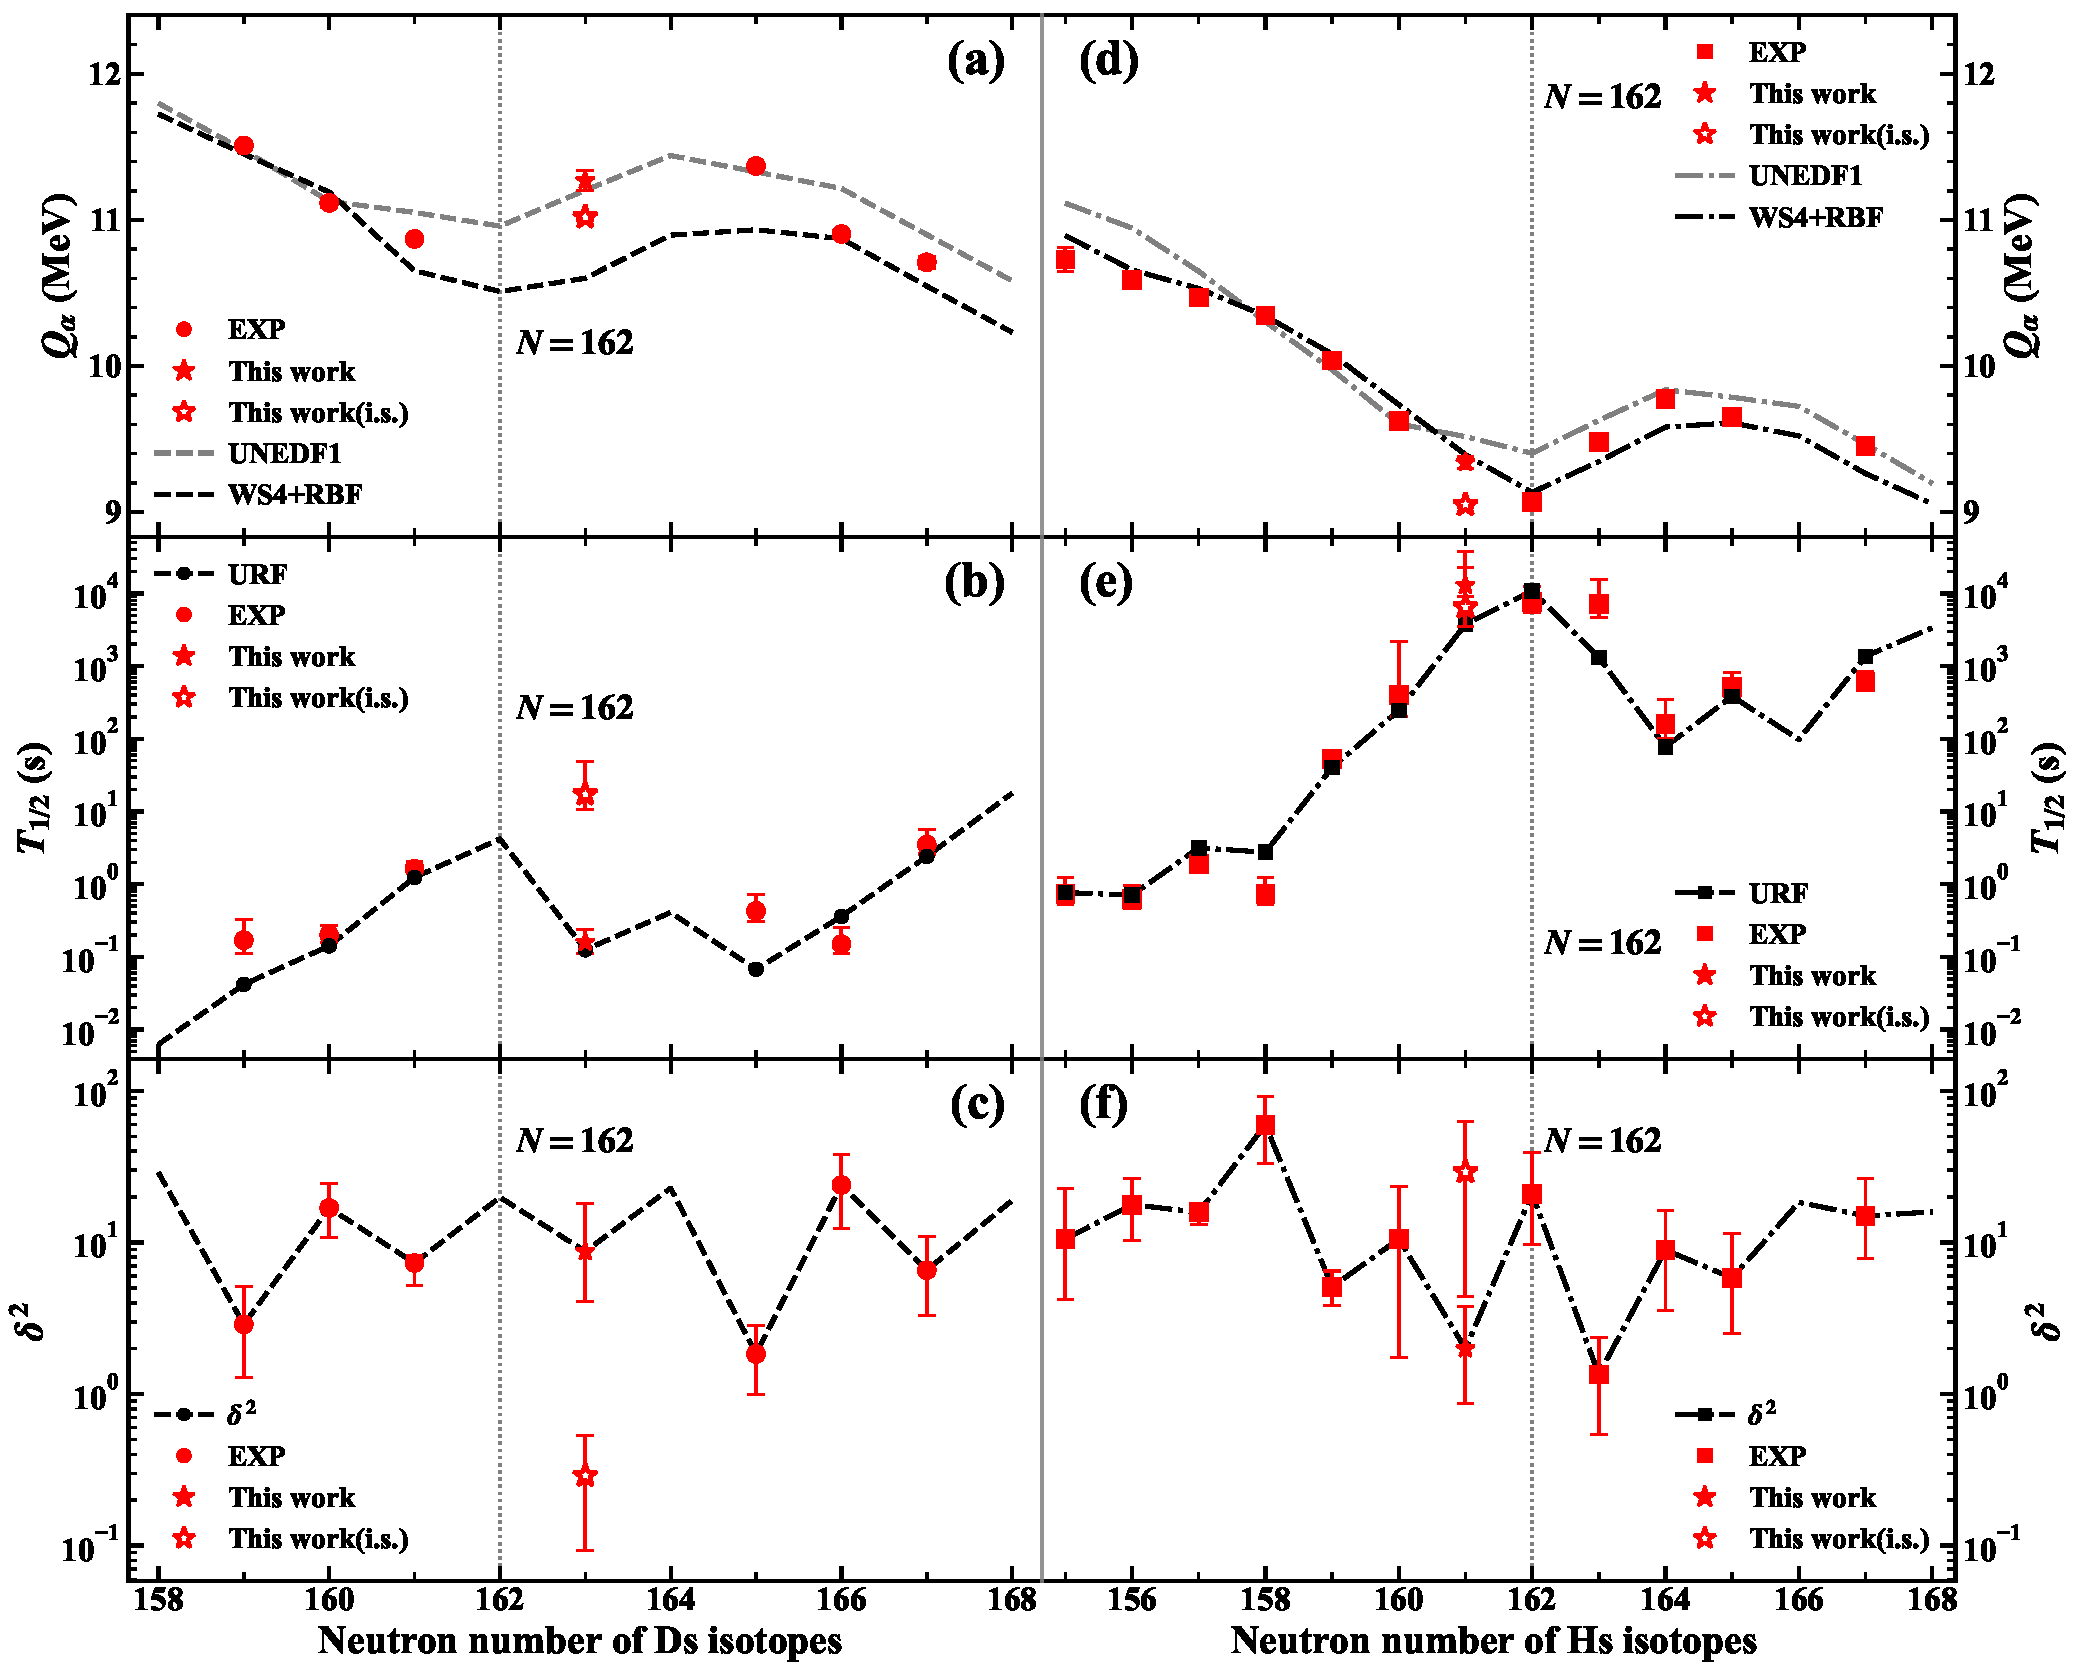
\includegraphics[width=0.95\textwidth]{System.pdf}
\caption{Ds 和 Hs 同位素链中 $Q_{\alpha}$、$T_{1/2}$ 以及约化 $\alpha$ 衰变宽度 $\delta^{2}$ 的系统学。图(a)--(c)对应 Ds 同位素，图(d)--(f)对应 Hs 同位素。上、中、下三排分别给出了 $Q_{\alpha}$、$T_{1/2}$ 和 $\delta^{2}$ 随中子数的变化。在 $Q_{\alpha}$ 图中，实验值与 UNEDF1 和 WS4+RBF 计算结果进行了比较；在半衰期图中，则与 URF 结果进行了比较。实心星号表示本文归属的支链，空心星号表示暂定的同核异能支链。竖直虚线表示 $N=162$。}
\label{fig:System}
\end{figure*}

考虑到形变 $N = 162$ 壳隙附近预期存在的壳结构，这一解释尤其值得关注 \cite{guoStabilizationDeformedSuperheavy2024}。核素 $^{273}$Ds 含有一个位于该壳隙之上的中子，而 $^{269}$Hs 则对应于该壳隙之下的一个中子空穴。因此，衰变链 $^{273}$Ds $\rightarrow$ $^{269}$Hs 实际上探测了同一个形变壳封闭两侧的单粒子结构。若干理论计算表明，在这一区域，低激发的高-$\Omega$ 中子组态可能起着重要作用。特别是，独宇称轨道 $\nu 13/2^{-}[716]$ 被预言靠近费米面，而对相邻奇-$N$ 锕后区核素的宏观—微观计算也将 $\nu 11/2^{-}[725]$ 列为低激发候选轨道之一 \cite{Shi2014,Parkhomenko2005}。在这种图像下，$^{273}$Ds 的长寿命支链可能与一种高-$\Omega$ 单中子组态有关。这种可能性在定性上也与邻近形变超重区中高-$K$ 同核异能现象的出现相一致，例如在 $^{270}$Ds $\rightarrow$ $^{266}$Hs 衰变序列中已有相关讨论 \cite{xuEnhancedStabilitySuperheavy2004}。然而，目前可获得的数据仍不足以给出唯一的自旋宇称或 Nilsson 轨道指认，因此仍存在多种可能解释。

在同样的框架下，子体核 $^{269}$Hs 中所观察到的衰变选择性也获得了自然的解释。若 $^{273}$Ds$^{a}$ 与 $^{273}$Ds$^{b}$ 对应不同的本征组态，则有利的 $\alpha$ 衰变应当优先布居具有相似结构的子体态。因此，在低能支链中出现、并与 $^{273}$Ds$^{a}$ 优先相关联的 $^{269}$Hs$^{c}$ 群，可能反映了子体核中相应的低激发组态。相较之下，较高能量的 $^{269}$Hs$^{a}$ 和 $^{269}$Hs$^{b}$ 两组，则可能与 $^{273}$Ds$^{b}$ 的衰变相关。从这个意义上说，本文数据所反映的可能不仅是 $^{273}$Ds 中存在同核异能结构，也可能是 $^{269}$Hs 中存在关联的多态结构。不过仍需强调的是，目前关于 $^{269}$Hs 存在三个不同分组的证据仍属暂定，尚不能排除部分观测到的模式实际上来源于未分辨的亚组。

同位素系统学也为这一图像提供了额外支持。如图~\ref{fig:System} 所示，Ds 和 Hs 同位素链中 $Q_{\alpha}$、半衰期以及约化 $\alpha$ 衰变宽度的演化，为本文的归属提供了更广阔的背景。在简单的单组态图像下，这些观测量通常应随中子数较为平滑地变化。局部支链分离，尤其是当它同时体现在衰变能、寿命和约化宽度上时，更自然地应被解释为结构变化的信号，而非统计涨落。在本文中，$^{273}$Ds 的长寿命支链和 $^{269}$Hs 的低能支链偏离了局域趋势，因此增强了其对应不同底层组态的解释。同时，在这一强形变超重区，约化宽度具有模型依赖性，因为形变、角动量变化以及结构效应都会进入其提取过程。基于这一原因，本文中约化宽度不应被视为同核异能态存在的独立证据。它的主要价值在于比较性：当在同一处方下自洽地加以评估时，它可以作为一个额外指标，表明所提出的几条支链在结构上确有差异。

\begin{figure}[htbp]
\centering
% 把下面文件名替换成你自己的图
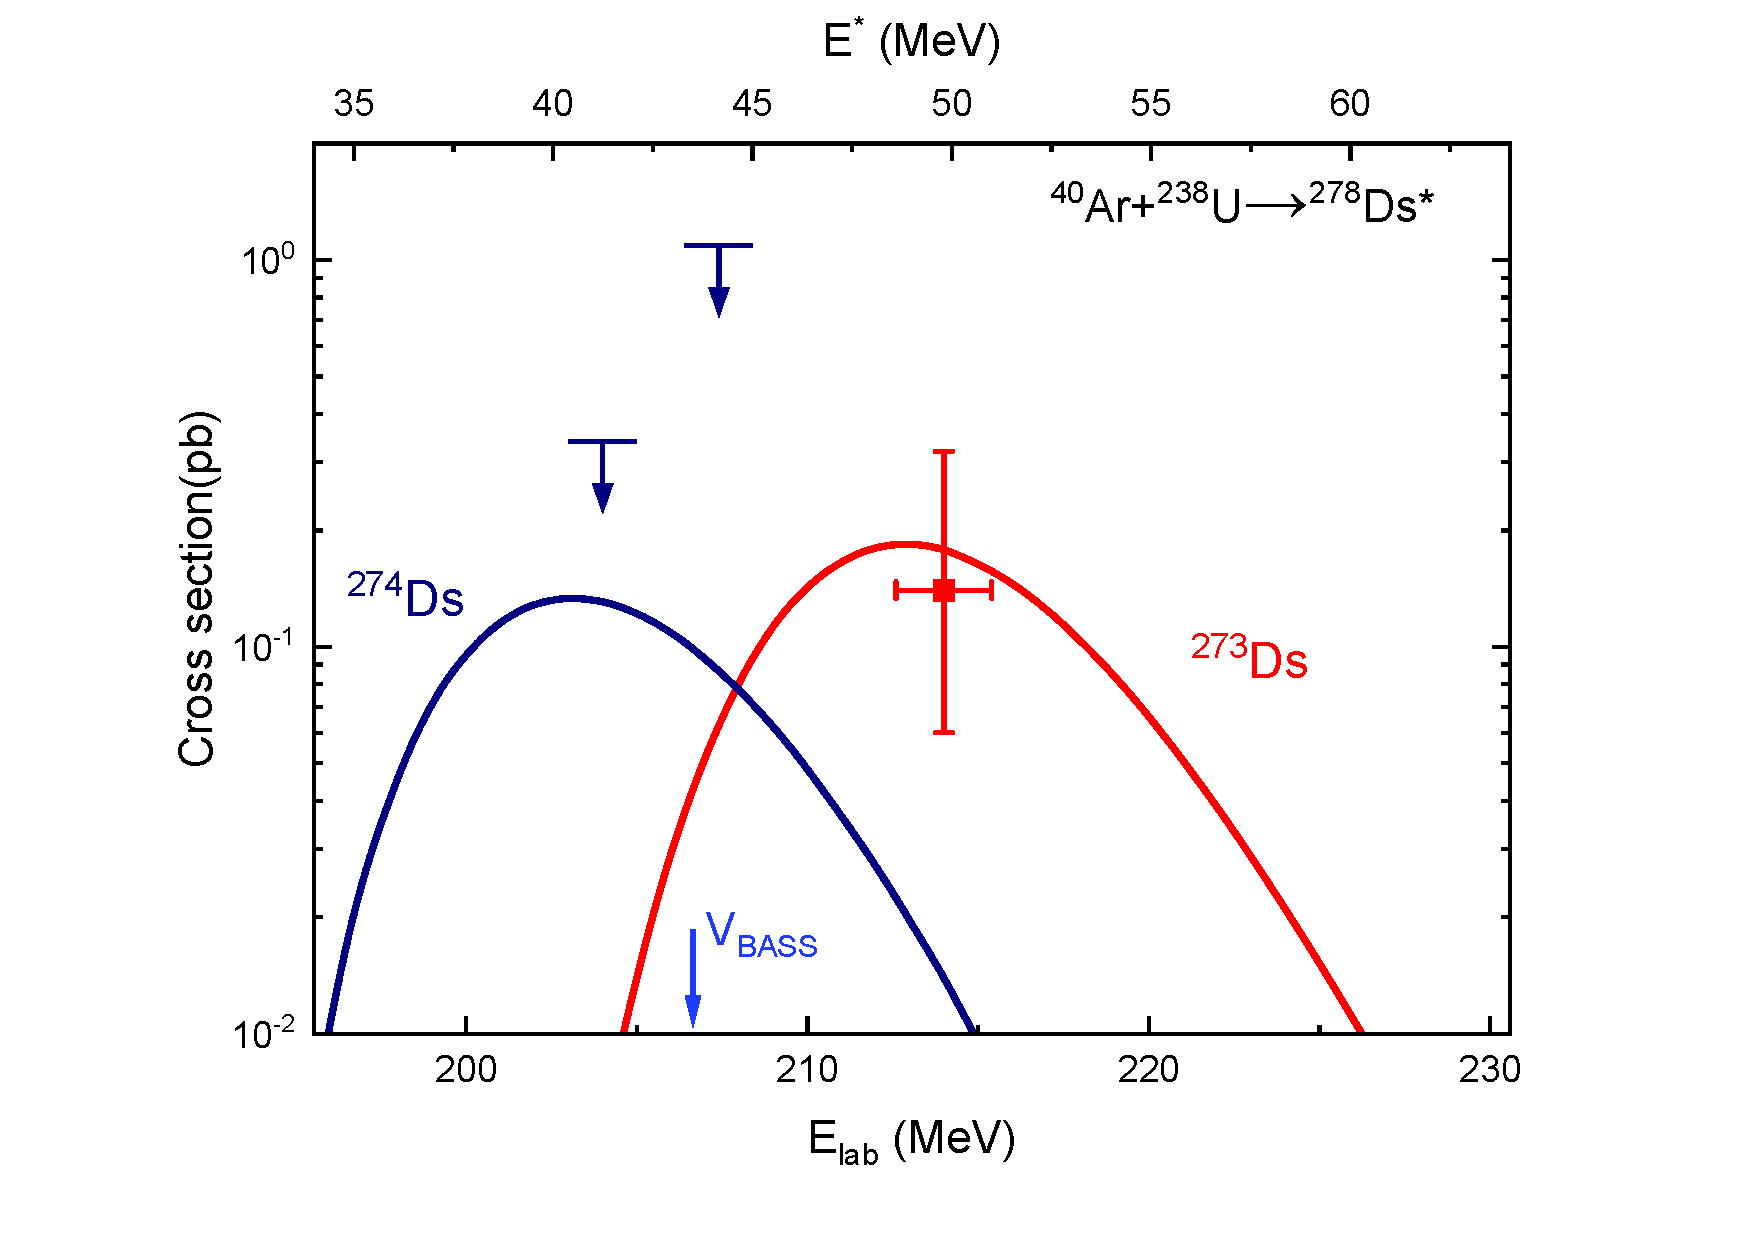
\includegraphics[width=0.62\textwidth]{exFun.pdf}
\caption{$^{40}$Ar + $^{238}$U $\rightarrow$ $^{278}$Ds$^{*}$ 反应的测量截面及其上限。曲线给出了通向 $^{274}$Ds 和 $^{273}$Ds 的 $4n$ 与 $5n$ 道的激发函数计算结果。下方横轴表示实验室系束流能量，上方横轴表示复合核对应的平均激发能。标注为 $V_{\mathrm{BASS}}$ 的箭头表示按照 BASS 经验公式估算得到的库仑势垒。}
\label{fig:exFun}
\end{figure}

激发函数的信息为本文的解释提供了进一步的一致性检验。如图~\ref{fig:exFun} 所示，在本文所采用的束流能量下，测得的截面与该能区 $5n$ 道占主导的计算预期总体一致。这一结果支持将所观测到的衰变链归属为通过 $^{238}$U($^{40}$Ar, $5n$)$^{273}$Ds 反应产生的 $^{273}$Ds，而不是归属于邻近蒸发道。尽管激发函数本身并不能区分不同的本征态，但它表明长寿命支链和短寿命支链是在同一个反应框架中出现的。这一点加强了如下结论：两条支链之间的差别更可能源于核结构本身，而不是来自不同反应道的混入。

\begin{thebibliography}{99}

\bibitem{oganessian2024SynthesisDecayProperties}
Y. T. Oganessian \textit{et al.},
Synthesis and decay properties of superheavy nuclei,
2024.

\bibitem{clark2023RoleQuasiparticleStructure}
R. M. Clark \textit{et al.},
Role of quasiparticle structure in $\alpha$ decay,
2023.

\bibitem{guoStabilizationDeformedSuperheavy2024}
J. G. Guo \textit{et al.},
Stabilization of deformed superheavy nuclei,
2024.

\bibitem{Shi2014}
Y. Shi \textit{et al.},
Low-lying quasiparticle structure in transfermium nuclei,
2014.

\bibitem{Parkhomenko2005}
A. Parkhomenko and A. Sobiczewski,
Structure of odd-$N$ transfermium nuclei,
2005.

\bibitem{xuEnhancedStabilitySuperheavy2004}
F. R. Xu \textit{et al.},
Enhanced stability in superheavy nuclei,
2004.

\end{thebibliography}

\end{document}